\documentclass[letterpaper,12pt,fleqn]{article}
\usepackage{matharticle}
\pagestyle{plain}
\renewcommand{\a}{\alpha}
\newcommand{\w}{\omega}
\begin{document}
Cavallaro, Jeffery \\
Math 221b \\
Homework \#6

\begin{enumerate}
\item Show that if $f:\C\to\R$ is a ring homomorphism then $f$ must be
  trivial.

  This is equivalent to saying that $\ker(f)=\C$. Since $\ker(f)$ must be ideal
  in $\C$, and since $\C$ is a field, any non-zero element in $\ker(f)$ is a
  unit and thus would cause $\ker(f)=\C$. Thus, the only two choices for
  $\ker(f)$ are the zero ideal and $\C$, where the latter means that the
  ring homomorphism is trivial. So, we want to eliminate the zero ideal as a
  possibility.

  So ABC that the kernel is trivial. This means that $f$ is injective. Now,
  let $z$ be a non-zero element of $\C$:
  \[f(z)=f(1z)=f(1)f(z)\]
  and since $f$ is injective and $f(0)=0$, neither $f(1)$ nor $f(z)$ can be
  0, and so $f(1)$ is the identity in $\R$ and so $f(1)=1$. But $\C$ and $\R$
  are additive groups so $f(-1)=-f(1)=-1$.

  Now, consider the following:
  \[f(i^2)=f(i)f(i)=f(i)^2=f(-1)=-f(1)=-1\]
  Thus, there exists some $x\in\R$ such that $x^2=-1$, a contradiction.

  Therefore, $\ker(f)=\C$ and $f$ is trivial.

  \bigskip

  \newcommand{\st}{\sqrt{3}}
  \newcommand{\ct}{\sqrt[3]{2}}
  \newcommand{\cf}{\sqrt[3]{4}}
  \newcommand{\fk}{\Q(\ct,\st)}
  \newcommand{\fl}{\Q(\ct)}
  \newcommand{\flt}{\Q(\st)}

\item Consider the field $K=\fk$ as an extension of $F=\Q$:
  \begin{enumerate}
  \item Show that $[K:F]=6$

    Consider the following field extensions:

    \begin{tikzpicture}
      \node (F) at (0,0) {$\Q$};
      \node (L) at (0,2) {$\fl$};
      \node (K) at (0,4) {$\fk$};
      \draw (F) to (L);
      \draw (L) to (K);
    \end{tikzpicture}

    Note that all of these extensions are algebraic.

    First, consider $\fl/\Q$ and the polynomial $f(x)=x^3-2\in\Q[x]$. By the rational
    root test, $f(x)$ is irreducible in $\Q$. Furthermore, $f(\ct)=0$, and thus
    $f(x)=m_{\ct,\Q}(x)$ and $[\fl:\Q]=3$:

    \begin{tikzpicture}
      \node (F) at (0,0) {$\Q$};
      \node (L) at (0,2) {$\fl$};
      \node (K) at (0,4) {$\fk$};
      \draw (F) to node [right] {$3$} (L);
      \draw (L) to (K);
    \end{tikzpicture}

    Next, consider $\fk/\fl$ and the polynomial $g(x)=x^2-3\in\fl[x]$. Since $g(\st)=0$,
    $m_{\st,\fl}(x)\mid g(x)$, and so $\deg(m_{\st,\fl}(x))=1$ or $2$.

    ABC: $\deg(m_{\st,\fl}(x))=1$ \\
    This would mean that $\fk=\fl$ and thus $\st\in\fl$. \\
    But that would mean that $Q\subset\flt\subset\fl$. \\
    So consider $g(x)=x^2-3\in\Q[x]$. By the rational root test, $g(x)$ is irreducible in
    $\Q$. Furthermore, $g(\st)=0$, and thus $g(x)=m_{\st,\Q}(x)$ and $[\flt:\Q]=2$.
    However, in order for $\flt\subset\fl$ it must be the case that
    $[\flt:\Q]\mid[\fl:\Q]$, but $2\nmid3$ - contradiction.

    Thus $\deg(m_{\st,\fl}(x))=2$ and so $[\fk:\fl]=2$:

    \begin{tikzpicture}
      \node (F) at (0,0) {$\Q$};
      \node (L) at (0,2) {$\fl$};
      \node (K) at (0,4) {$\fk$};
      \draw (F) to node [right] {$3$} (L);
      \draw (L) to node [right] {$2$} (K);
    \end{tikzpicture}

    Therefore, $[\fk:\Q]=[\fk:\fl][\fl:\Q]=2\cdot3=6$

    \bigskip

  \item Find a primitive element $\a$ for $K/F$.

    \newcommand{\fa}{\Q(\st+\ct)}

    Let $\a=\st+\ct\in K/F$. \\
    We need to show that $\fk=\fa$.
    Consider the factors:
    
    $a_1(x)=[x-(\st+\ct)]$ \\
    $a_2(x)=[x-(-\st+\ct)]$ \\
    $a_3(x)=[x-(\st+\w\ct)]$ \\
    $a_4(x)=[x-(-\st+\w\ct)]$ \\
    $a_5(x)=[x-(\st+\w^2\ct)]$ \\
    $a_6(x)=[x-(-\st+\w^2\ct)]$

    All of these factors need to be applied in order to obtain a polynomial with
    coefficients in $\Q$:
    
    $f(x)=a_1(x)a_2(x)a_3(x)a_4(x)a_5(x)a_6(x)=x^6-9x^4-4x^3+27x^2-36x-23$

    But $\fa$ is a UFD, and so $f(x)$ is irreducible in $\Q$. Also, $f(\st+\ct)=0$,
    and so $f(x)=m_{\st+\ct,\Q}(x)$, and thus $[\fa:\Q]=6$. But $\st+\ct\in\fk$, so
    $\Q\subset\fa\subset\fk$

    Therefore $\fa=\fk$.
  \end{enumerate}

  \bigskip

\item Suppose $K/F$ is an algebraic extension of fields. Prove that if $R$ is a ring
  with $F\subseteq R\subseteq K$ then $R$ must also be a field.

  It suffices to show that $R^*$ is closed under multiplicative inverses.
  
  Assume $\a\in R^*$ \\
  Since $K/F$ is an algebraic extension and $\a\in K$, $\a$ is algebraic over $F$.
  Thus, there is guaranteed to be an algebraic extension $F(\a)/F$ such that
  $F\subseteq F(\a)\subseteq R\subseteq K$. But $F(\a)$ is a field and so
  $\a^{-1}\in F(\a)\in R$.

  \bigskip

\item Let $K/F$ be a field extension and supposed $\a\in K$ is algebraic over $F$.
  Show that if $\deg(m_{\a,F}(x))$ is odd then $F(\a^2)=F(\a)$.

  If $\a\in F$ then done, so AWLOG: $\a\notin F$.

  Assume $\deg(m_{\a,F}(x))$ is odd, and thus $[F(\a):F]$ is odd. \\
  ABC: $F(\a^2)\ne F(\a)$. \\
  This means that $\a\notin F(\a^2)$, but $F(\a)$ is a ring so $\a^2\in F(\a)$. So
  consider the following extensions:

  \begin{tikzpicture}
    \node (F) at (0,0) {$F$};
    \node (L) at (0,2) {$F(\a^2)$};
    \node (K) at (0,4) {$F(\a)$};
    \draw (F) to (L);
    \draw (L) to (K);
  \end{tikzpicture}

  Since $\a$ is a root of $x^2-\a^2$, this means that $[F(\a):F(\a^2)]\le2$. But since
  $\a\notin F(\a^2)$ this means that $[F(\a):F(\a^2)]\ge2$. Thus
  $[F(\a):F(\a^2)]=2$:

  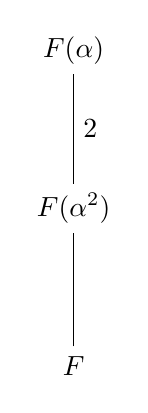
\begin{tikzpicture}
    \node (F) at (0,0) {$F$};
    \node (L) at (0,2) {$F(\a^2)$};
    \node (K) at (0,4) {$F(\a)$};
    \draw (F) to (L);
    \draw (L) to node [right] {$2$} (K);
  \end{tikzpicture}

  Thus, $[F(\a):F]$ has a power of 2 in it and must be even - contradiction.

  Therefore, $F(\a^2)=F(\a)$.

  \bigskip

  \newcommand{\fw}{Q(\ct,\w)}
  
\item Find the splitting field $K\subseteq\C$ for $x^3-2$ over $\Q$ and
  determine all subfields of $K$.
  
  First, find all roots of $x^3-2$ in $\C$:
  \[x^3=2=2e^{i2\pi n}\]
  \[x=\ct e^{i\frac{2\pi}{3}n}\]
  \[x=\ct,\ct\w,\ct\w^2\]
  And therefore $x^3-2$ splits in $\fw$.

  We have already showed that $[\fl:\Q]=3$, so consider the field extensions:

  \begin{tikzpicture}
    \node (F) at (0,0) {$\Q$};
    \node (L) at (0,2) {$\fl$};
    \node (K) at (0,4) {$\fw$};
    \draw (F) to node [right] {$3$} (L);
    \draw (L) to (K);
  \end{tikzpicture}

  Since $x^3-2$ has 3 roots in $\fw$ we know that $[\fw:\Q]\le3!=6$. But clearly
  $\w\notin\fl$ and so $\fl$ is properly contained in $\fw$. Since $[\fl:\Q]=3$ must
  divide $[\fw:\Q]$, which can only be $4$, $5$, or $6$, this forces $[\fw:\Q]=6$.

  The subfields are derived from the roots. Guard against duplicates:

  $\ct,\cf$ \\
  $\w,\w^2$ \\
  $\w\ct,\w^2\cf$ \\
  $\w^2\ct,\w\cf$ \\
  
  \begin{tikzpicture}
    \node (F) at (4,0) {$\Q$};
    \node (L1) at (0,4) {$\fl$};
    \node (L2) at (2,4) {$\Q(\w\ct)$};
    \node (L3) at (4,4) {$\Q(\w^2\ct)$};
    \node (L4) at (7,2) {$\Q(\w)$};
    \node (K) at (4,6) {$\fw$};
    \draw (F) to node [left] {$3$} (L1);
    \draw (F) to node [right] {$3$} (L2);
    \draw (F) to node [right] {$3$} (L3);
    \draw (F) to node [right] {$2$} (L4);
    \draw (L1) to node [left] {$2$} (K);
    \draw (L2) to node [left] {$2$} (K);
    \draw (L3) to node [left] {$2$} (K);
    \draw (L4) to node [right] {$3$} (K);
  \end{tikzpicture}

\end{enumerate}

\end{document}
